In order to test the performance of the discrete controller, it has been implemented on the continuous time linear system (SIMULINK model figure \ref{fig:modelp16}).

As we can see figure \ref{fig:p16d0} and figure \ref{fig:p16d}, the controller works well, that is to say, the reference position is well followed. Indeed, with or without the noise \textbf{d}, the tracking is the same, with a dilay $\tau = 0.0026\ s$

\begin{figure}[H]
 \centering 
 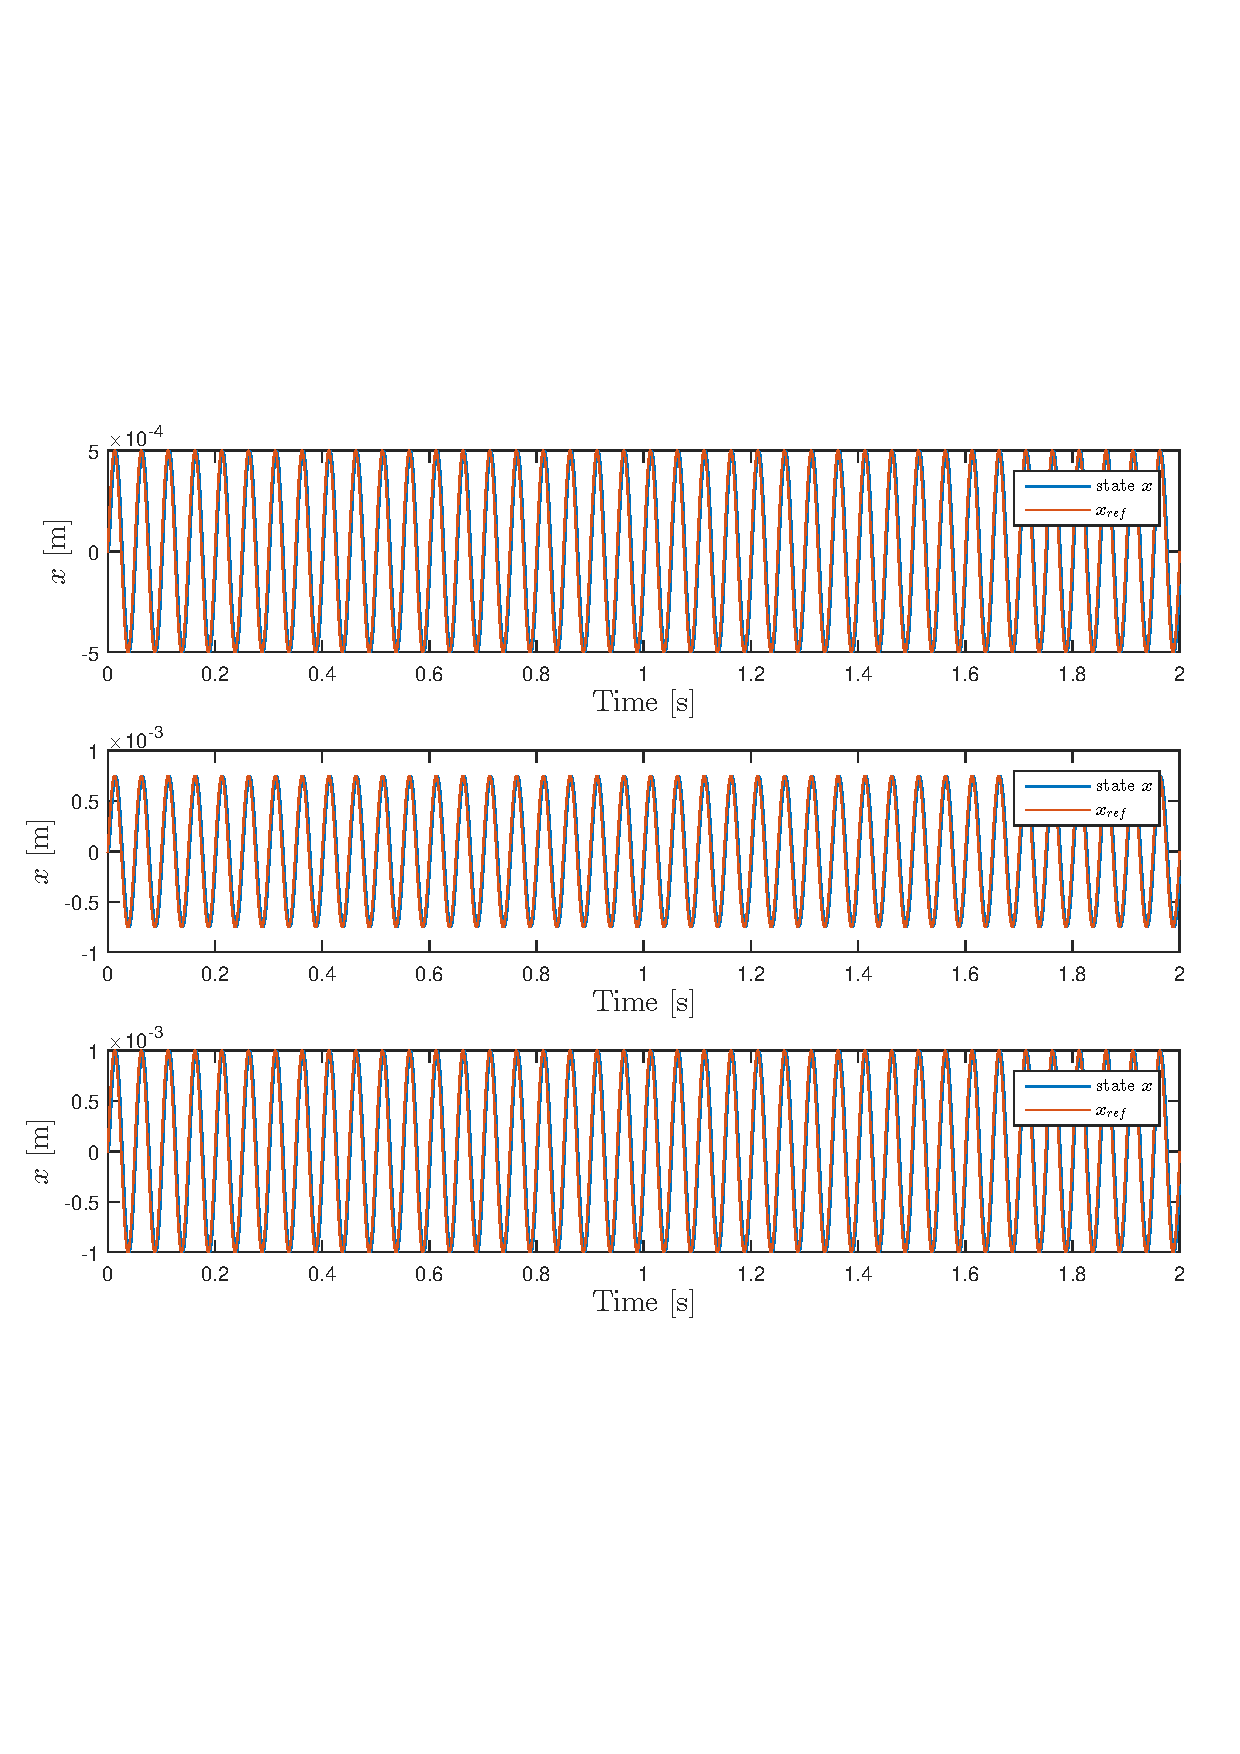
\includegraphics[trim=2cm 7cm 2cm 7cm, clip=true, totalheight=0.35\textheight, angle=0]{figures/p16d0.pdf}
 \caption{response of the state x to the input $x_{ref}$ with $Ax = [0.0005,0.00075, 0.001]$ (from the top to the bottom) with the controller without noise}
 \label{fig:p16d0}
\end{figure}

\begin{figure}[H]
 \centering 
 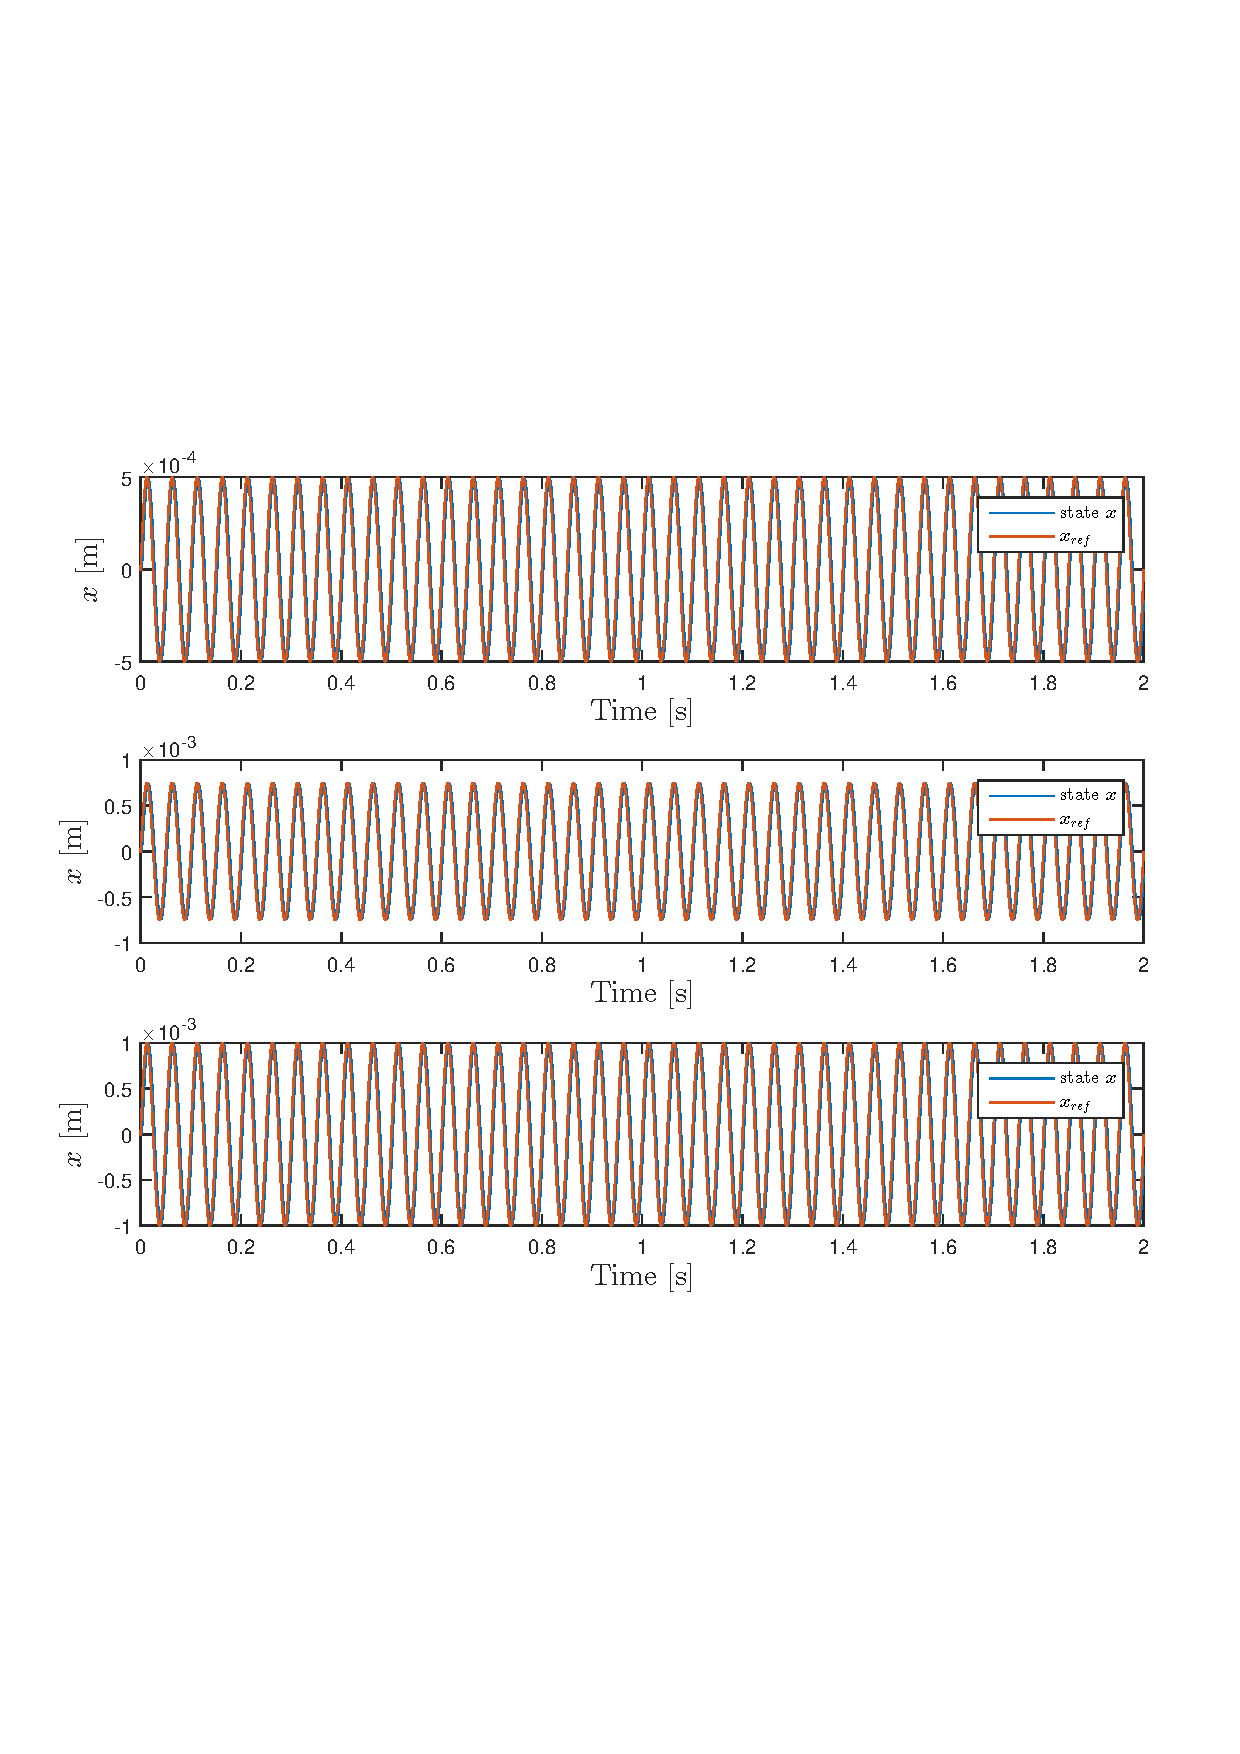
\includegraphics[trim=2cm 7cm 2cm 7cm, clip=true, totalheight=0.35\textheight, angle=0]{figures/p16d.pdf}
 \caption{response of the state x to the input $x_{ref}$ with $Ax = [0.0005,0.00075, 0.001]$ (from the top to the bottom) with the controller with the noise \textbf{d}}
 \label{fig:p16d}
\end{figure}

We can notice that it is odd that there is no difference between the simulation with or without the noise \textbf{d}.